\section{Forecasting Methodology}
\label{sec:methodology}

\subsection{Probabilistic Forecasting Formulation}
\label{subsec:probabilistic}

The forecasting task is formulated probabilistically through conditional
quantile estimation. Rather than predicting a single future traffic speed,
the neural forecasting models estimate three quantiles for each sensor and
forecasting step,

\begin{equation}
    \mathcal{Q} = \{0.1, 0.5, 0.9\}.
    \label{eq:quantiles}
\end{equation}

For an input window $\mathbf{X}_t$, the models therefore produce

\begin{equation}
    \hat{\mathbf{Y}}_t
    \in
    \mathbb{R}^{F \times N \times |\mathcal{Q}|},
    \label{eq:probabilistic_output}
\end{equation}

where $F=12$ is the forecasting window, $N=207$ is the number of sensors,
and $|\mathcal{Q}|=3$ is the number of predicted quantiles.

The median prediction $\hat{y}^{(0.5)}$ is used as the point forecast when
computing deterministic metrics such as MAE and RMSE. The lower and upper
quantiles define the predictive interval

\begin{equation}
    \left[
        \hat{y}^{(0.1)},
        \hat{y}^{(0.9)}
    \right],
    \label{eq:prediction_interval}
\end{equation}

which has a nominal coverage probability of $80\%$. This formulation makes it
possible to evaluate point forecasting accuracy and predictive uncertainty
using a single model.


The models are trained using the Pinball Loss. For a target value $y$, a
predicted quantile $\hat{y}^{(q)}$, and a quantile level $q$, the loss is
defined as

\begin{equation}
    \mathcal{L}_{q}
    \left(y,\hat{y}^{(q)}\right)
    =
    \max
    \left(
        q\left(y-\hat{y}^{(q)}\right),
        (q-1)\left(y-\hat{y}^{(q)}\right)
    \right).
    \label{eq:pinball_loss}
\end{equation}

Unlike a symmetric regression loss, the Pinball Loss penalizes
underestimation and overestimation differently according to the target
quantile. Minimizing it therefore allows the model to estimate different
regions of the conditional target distribution rather than only its central
value.


Since some target observations are unavailable, the Pinball Loss is computed
only over valid target entries. During training, consider a mini-batch of
$B$ samples. Let $b \in \{1,\ldots,B\}$ denote the sample index,
$h \in \{1,\ldots,F\}$ the forecast step, and
$n \in \{1,\ldots,N\}$ the sensor index. The binary mask
$m_{b,h,n} \in \{0,1\}$ indicates whether the corresponding target value is
available.

For each mini-batch, the training loss is obtained by averaging the Pinball
Loss over all valid target entries and over all predicted quantiles:

\begin{equation}
    \mathcal{L}_{\mathrm{masked}}
    =
    \frac{
        \displaystyle
        \sum_{b=1}^{B}
        \sum_{h=1}^{F}
        \sum_{n=1}^{N}
        m_{b,h,n}
        \sum_{q\in\mathcal{Q}}
        \mathcal{L}_{q}
        \left(
            y_{b,h,n},
            \hat{y}_{b,h,n}^{(q)}
        \right)
    }{
        \displaystyle
        |\mathcal{Q}|
        \sum_{b=1}^{B}
        \sum_{h=1}^{F}
        \sum_{n=1}^{N}
        m_{b,h,n}
    }.
    \label{eq:masked_pinball}
\end{equation}

Consequently, unavailable target values do not contribute to the loss,
while every valid target contributes once for each quantile in
$\mathcal{Q}$. This is consistent with the missing-data strategy described
in Section~\ref{subsec:missing}.


\subsection{Persistence Baseline}
\label{subsec:persistence}

A persistence model is used as the simplest forecasting baseline. For each
sensor, the value at the final time step of the input window is repeated
across the complete forecasting horizon. The prediction for sensor $n$ at
any future step $h$ is therefore

\begin{equation}
    \hat{y}_{t+h,n} = x_{t,n},
    \qquad h=1,\ldots,F.
    \label{eq:persistence}
\end{equation}

The persistence baseline contains no trainable parameters and does not
explicitly model either temporal dynamics or spatial interactions. It
therefore provides a simple reference for determining whether the learned
models extract useful predictive information from the historical traffic
sequence.


\subsection{Temporal GRU}
\label{subsec:gru}

The first learned forecasting model is a temporal GRU designed to capture
temporal dependencies without exploiting the sensor graph. Each sensor is
processed independently using its own sequence of historical traffic
observations, while the GRU parameters are shared across all sensors.

For a given sensor $n$, the input sequence

\begin{equation}
    \left[
        \tilde{x}_{t-H+1,n},
        \ldots,
        \tilde{x}_{t,n}
    \right]
\end{equation}

is processed by the same recurrent network. No information from other
sensors is exchanged during the forward pass. The model therefore provides a
controlled no-graph baseline against which the contribution of spatial
message passing can be evaluated.

The selected temporal architecture consists of a two-layer GRU with hidden
dimension 64. The final hidden representation of each sensor is passed to a
linear output layer that jointly predicts all $F=12$ future steps and all
three quantiles. For each sensor, the output layer therefore produces

\begin{equation}
    F \times |\mathcal{Q}| = 12 \times 3 = 36
\end{equation}

values, which are reshaped into the corresponding forecast-step and quantile
dimensions.

The complete model contains 40164 trainable parameters. Because the same
network is applied to every sensor, the parameter count does not scale with
the number of nodes in the traffic network.


\subsection{Graph Representation and Diffusion Message Passing}
\label{subsec:graph}

Spatial dependencies are introduced through the sensor graph provided with
METR-LA. Each traffic sensor corresponds to a graph node, while the adjacency
matrix

\begin{equation}
    \mathbf{A} \in \mathbb{R}^{N \times N}
\end{equation}

encodes directed, weighted connections between sensors. Throughout this work,
the convention is that $A_{ij}$ represents the weight assigned at node $i$
to the message received from node $j$. Therefore, row $i$ contains the
weights used to aggregate information into node $i$.

The provided adjacency matrix already contains self-connections. Therefore,
no additional identity matrix is added to $\mathbf{A}$ before normalization.
This avoids introducing artificial self-loops or modifying the relative
weights of the graph supplied with the dataset.

Before message passing, the adjacency matrix is row-normalized as

\begin{equation}
    \mathbf{P} = \mathbf{D}^{-1}\mathbf{A},
    \label{eq:row_normalization}
\end{equation}

where $\mathbf{D}$ is the diagonal matrix of row sums,

\begin{equation}
    D_{ii} = \sum_j A_{ij}.
\end{equation}

Under the adopted convention, the one-step propagated representation of node
$i$ is therefore

\begin{equation}
    (\mathbf{P}\mathbf{X})_i
    =
    \sum_j P_{ij}\mathbf{X}_j,
    \label{eq:graph_aggregation}
\end{equation}

so that node $i$ receives a weighted combination of the representations of
the nodes $j$ connected to it.

Spatial information is propagated through a diffusion-style message-passing
layer. Given node features $\mathbf{X}$, the layer computes

\begin{equation}
    \mathbf{H}
    =
    \sum_{k=0}^{K}
    \mathbf{P}^{k}\mathbf{X}\mathbf{W}_{k}
    +
    \mathbf{b},
    \label{eq:diffusion}
\end{equation}

where $K$ controls the maximum diffusion depth and each $\mathbf{W}_{k}$ is
a learnable projection associated with a different propagation step. The
$k=0$ term, for which $\mathbf{P}^{0}=\mathbf{I}$, directly preserves the
node's own representation, while the terms with $k\geq1$ incorporate
information propagated through the graph.

For the main configuration, $K=2$, yielding

\begin{equation}
    \mathbf{H}
    =
    \mathbf{X}\mathbf{W}_{0}
    +
    \mathbf{P}\mathbf{X}\mathbf{W}_{1}
    +
    \mathbf{P}^{2}\mathbf{X}\mathbf{W}_{2}
    +
    \mathbf{b}.
    \label{eq:diffusion_k2}
\end{equation}

The first term provides an explicit transformation of each node's own
representation, while the remaining terms incorporate information propagated
over one and two graph transitions. Since the diagonal entries already
present in $\mathbf{A}$ are preserved by the row normalization, the
one-step and two-step diffusion terms may themselves also contain
self-information.


\subsection{Graph-Temporal Architecture}
\label{subsec:graph_temporal}

The main forecasting model combines the diffusion operation described in
Section~\ref{subsec:graph} with recurrent temporal modeling. The architecture
is composed of two consecutive graph-temporal blocks. Each block first
propagates information between sensors through diffusion message passing and
then applies a GRU to model the temporal evolution of the resulting node
representations (Figure \ref{fig:graphtemporalarchitecture}).

Given an input window, diffusion is applied independently at each temporal
step, allowing every sensor representation to incorporate information from
its graph neighborhood. The resulting sequence of spatial representations is
then processed by a GRU independently for each node, with recurrent
parameters shared across sensors. The first block preserves the complete
temporal sequence so that it can be processed by the second diffusion--GRU
block.

The final temporal representation is passed to a linear probabilistic head
that directly predicts the 12 future steps for the three quantile levels
defined in Section~\ref{subsec:probabilistic}. As in the Temporal GRU, the
complete forecasting window is generated in a single forward pass rather
than recursively feeding previous predictions back into the model.

The selected graph-temporal model uses a graph hidden dimension of 64, a GRU
hidden dimension of 64, one GRU layer per graph-temporal block, two
graph-temporal blocks, and a diffusion depth of $K=2$. The complete
architecture contains 64868 trainable parameters.

\begin{figure}[t]
    \centering
    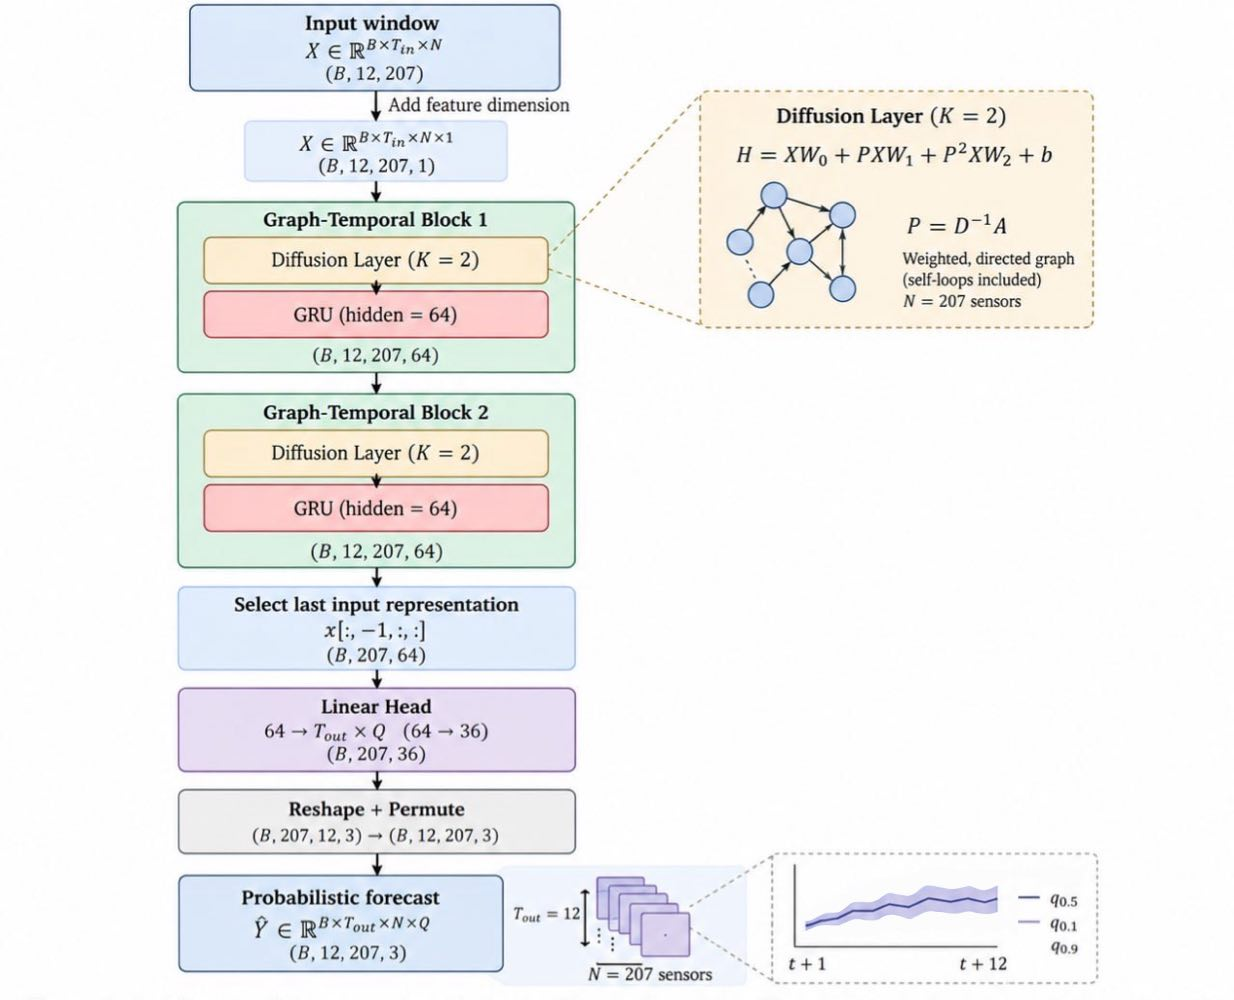
\includegraphics[width=\linewidth]{img/graphtemporalarchitecture}
    \caption{Architecture of the proposed graph-temporal forecasting model.}
    \label{fig:graphtemporalarchitecture}
\end{figure}